\documentclass[openany]{article}
\usepackage{lmodern}
\usepackage{amssymb,amsmath}
\usepackage{ifxetex,ifluatex}
\usepackage{fixltx2e} % provides \textsubscript
\ifnum 0\ifxetex 1\fi\ifluatex 1\fi=0 % if pdftex
  \usepackage[T1]{fontenc}
  \usepackage[utf8]{inputenc}
\else % if luatex or xelatex
  \ifxetex
    \usepackage{mathspec}
  \else
    \usepackage{fontspec}
  \fi
  \defaultfontfeatures{Ligatures=TeX,Scale=MatchLowercase}
\fi
% use upquote if available, for straight quotes in verbatim environments
\IfFileExists{upquote.sty}{\usepackage{upquote}}{}
% use microtype if available
\IfFileExists{microtype.sty}{%
\usepackage{microtype}
\UseMicrotypeSet[protrusion]{basicmath} % disable protrusion for tt fonts
}{}
\usepackage{hyperref}
\hypersetup{unicode=true,
            pdftitle={Systems Pathology: Eye and Ear},
            pdfauthor={Russell Fraser},
            pdfborder={0 0 0},
            breaklinks=true}
\urlstyle{same}  % don't use monospace font for urls
\usepackage{natbib}
\bibliographystyle{apalike}
\usepackage{longtable,booktabs}
\usepackage{graphicx,grffile}
\makeatletter
\def\maxwidth{\ifdim\Gin@nat@width>\linewidth\linewidth\else\Gin@nat@width\fi}
\def\maxheight{\ifdim\Gin@nat@height>\textheight\textheight\else\Gin@nat@height\fi}
\makeatother
% Scale images if necessary, so that they will not overflow the page
% margins by default, and it is still possible to overwrite the defaults
% using explicit options in \includegraphics[width, height, ...]{}
\setkeys{Gin}{width=\maxwidth,height=\maxheight,keepaspectratio}
\IfFileExists{parskip.sty}{%
\usepackage{parskip}
}{% else
\setlength{\parindent}{0pt}
\setlength{\parskip}{6pt plus 2pt minus 1pt}
}
\setlength{\emergencystretch}{3em}  % prevent overfull lines
\providecommand{\tightlist}{%
  \setlength{\itemsep}{0pt}\setlength{\parskip}{0pt}}
\setcounter{secnumdepth}{5}
% Redefines (sub)paragraphs to behave more like sections
\ifx\paragraph\undefined\else
\let\oldparagraph\paragraph
\renewcommand{\paragraph}[1]{\oldparagraph{#1}\mbox{}}
\fi
\ifx\subparagraph\undefined\else
\let\oldsubparagraph\subparagraph
\renewcommand{\subparagraph}[1]{\oldsubparagraph{#1}\mbox{}}
\fi

%%% Use protect on footnotes to avoid problems with footnotes in titles
\let\rmarkdownfootnote\footnote%
\def\footnote{\protect\rmarkdownfootnote}

%%% Change title format to be more compact
\usepackage{titling}

% Create subtitle command for use in maketitle
\providecommand{\subtitle}[1]{
  \posttitle{
    \begin{center}\large#1\end{center}
    }
}

\setlength{\droptitle}{-2em}

  \title{Systems Pathology: Eye and Ear}
    \pretitle{\vspace{\droptitle}\centering\huge}
  \posttitle{\par}
    \author{Russell Fraser}
    \preauthor{\centering\large\emph}
  \postauthor{\par}
      \predate{\centering\large\emph}
  \postdate{\par}
    \date{2020-03-13}

\usepackage{booktabs}
\usepackage{booktabs}
\usepackage{longtable}
\usepackage{array}
\usepackage{multirow}
\usepackage{wrapfig}
\usepackage{float}
\usepackage{colortbl}
\usepackage{pdflscape}
\usepackage{tabu}
\usepackage{threeparttable}
\usepackage{threeparttablex}
\usepackage[normalem]{ulem}
\usepackage{makecell}
\usepackage{xcolor}

\begin{document}
\maketitle

{
\setcounter{tocdepth}{2}
\tableofcontents
}
\section*{About}\label{about}
\addcontentsline{toc}{section}{About}

These notes are a fairly comprehensive collection of information to
complement the lectures and labs delivered in VETM2220, Systems
Pathology II, on the topic of the pathology of the eye and ear. Although
all of the information is useful, certain areas will have been
emphasized in lecture, let the areas focused on in lectures and lab
guide your studying. There are a few rare conditions that are not
discussed in these notes, and you are encouraged to read through the
relevant chapters in the textbooks recommended below.

Unfortunately, there are only three lectures assigned to this topic,
barely enough time to begin scraping the surface of eye and ear
pathology. Reviewing these notes will be critical, and they will
hopefully help serve as a reference when you are in practice. Diseases
of the eye and ear are \textbf{very} commonly encountered, especially in
small animal practice. Developing a good understanding of the
pathogenesis of the various ocular and aural conditions will serve you
well as a practitioner for years to come.

The notes are available online at \url{http://russfraser.ca/eye-ear/},
as a PDF on Moodle, and as an Epub (E-book format, suitable for a
tablet). Please feel free to provide feedback, whether on content,
style, or typos!

\subsubsection*{Contact me}\label{contact-me}
\addcontentsline{toc}{subsubsection}{Contact me}

Please don't hesitate to get in touch if you have any questions.

\begin{itemize}
\tightlist
\item
  Phone: 902-620-5183
\item
  E-mail: \href{mailto:rufraser@upei.ca}{\nolinkurl{rufraser@upei.ca}}
\item
  Office: 414N, Dept. of Pathology and Microbiology
\end{itemize}

\subsection*{Reference material}\label{reference-material}
\addcontentsline{toc}{subsection}{Reference material}

\begin{itemize}
\tightlist
\item
  Zachary, J. F., \& McGavin, M. D. (2016). Pathologic Basis of
  Veterinary Disease Expert Consult. Elsevier Health Sciences.
\item
  Maxie, G. (2015). Jubb, Kennedy \& Palmer's Pathology of Domestic
  Animals-E-Book (Vol. 1). Elsevier Health Sciences.
\end{itemize}

\subsection*{Acknowledgements}\label{acknowledgements}
\addcontentsline{toc}{subsection}{Acknowledgements}

These lecture notes were prepared in R \citep{R-base} using the bookdown
\citep{xie2015}, knitr \citep{R-knitr}, and Rmarkdown
\citep{R-rmarkdown} packages. Source material was taken from
\citet{zachary2016pathologic}, \citet{dubielzig}, \citet{histobasis},
and \citet{maxie2015jubb}. I gratefully acknoweldge the prior course
notes from Dr.~Pierre-Yves Daoust. Images are attributed throughout the
text; unattributed images are either mine or were found in the public
domain.

\section{Introduction to pathology of the eye}\label{intro}

The eye is a complex, unique structure, and a thorough description of
the anatomy and physiology of the eye is far beyond the scope of these
notes. An excellent summary is available in Chapter 21, p.~1269-1282 of
the reference textbook (Zachary and McGavin), and I strongly encourage
you to read it. A PDF copy of the chapter is available in Moodle. It
will help provide a solid foundation that will allow you to
\emph{understand} the development of ocular disease, rather than simply
memorizing the steps and lesions involved.

It is important to understand that the eye is a unique, highly organized
structure, and that disruptions to the delicate structures of the globe
can have \textbf{significant and severe consequences to the health of
the eye and to vision}. Furthermore, the globe is a \textbf{closed
system}, often sparing it from systemic insult, but also depriving it of
quick and efficient resolution from damaging events like inflammation or
hemorrhage. Recall that, like the brain and the testes, the eye has a
form of immune privilege. There are relatively few resident leukocytes,
leading to a relative delay in the onset of inflammation. Regeneration
and repair is similarly limited in comparison to other tissues. Finally,
unlike the liver or other tissues were parenchymal cells can divide and
regenerate functional organ mass following injury, the \textbf{eye has
very little regenerative potential}. Thus, \textbf{any damage} is of
consequence to the eye.

Most of what we will deal with in this section is the pathogenesis and
theory of disease. Where possible, we will look at the gross correlates,
but many of the conditions are better appreciated with an
ophthalmological exam, requiring specialized tools and techniques.
Microscopic images will be used to help reinforce concepts and provide a
visual correlate to the theory.

What follows in this chapter is a \emph{minimal} review of the basics of
ocular anatomy as it relates to pathology, to help refresh your memory
after having read the textbook. I've also put together a general
\protect\hyperlink{glossary}{Glossary} to help keep track of all the
terms that are unique to ocular pathology and ophthalmology, and which
seem to make up a language of their own.

\hypertarget{ocular-anatomy}{\subsection{Ocular
anatomy}\label{ocular-anatomy}}

A schematic of the eye is show in Figure \ref{fig:globe}. The globe is
surrounded by muscular tissue, eyelids, and a bony orbit. The globe
itself is made up of three conceptual layers: the sclera, which is
modified at its anterior end to become the cornea; the choroid, a
portion of the vascular supply of the eye; and the retina, the light
sensing interior layer. The choroid is continuous with the iris and
ciliary body. The lens, a structure designed to refract light, is
suspended by zonules originating from the ciliary body. These structures
create several compartments within the eye: the anterior chamber,
posterior chamber, and vitreous humour. Each of these structures is
complex and reacts to injury and disease in somewhat different ways.

\begin{figure}

{\centering 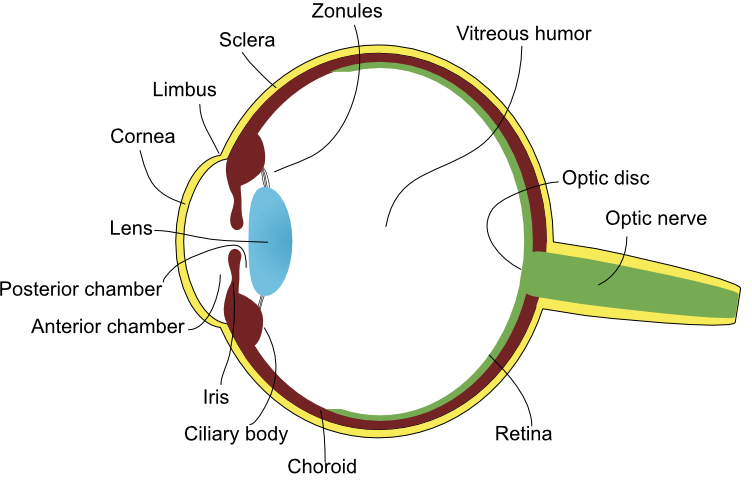
\includegraphics[width=0.6\linewidth]{images/globe-labeled} 

}

\caption{Cartoon of the globe illustrating many of the important anatomical structures. Note that the uvea is composed of the structures coloured red (the iris, ciliary body, and choroid).}\label{fig:globe}
\end{figure}

The eyelids are covered on one side by haired skin, which is
histologically similar to skin found in other areas. The other side is
covered by conjunctival epithelium, known as the palpebral conjunctiva.
Tear film, composed of mucous and fluid, is present between the bulbar
and palpebral conjunctiva, and is distributed through the action of
blinking. The eyelid margin is where the anterior haired surface and
posterior palpebral conjunctiva meet. Cilia, or eyelashes, are present
at the eyelid margin, along with a row modified sebaceous glands called
\textbf{meibomian or tarsal glands}.

The eyelids help protect the eye from physical injury and help remove
irritating contaminants from the surface of the eye. The tear film also
contains antibacterial peptides. The eyelids respond to injury in much
the same way as skin elsewhere in the body responds to injury. Given
their role in keeping the eye protected and moist, however, damage
resulting in defective function or congenital malformations (for
example, \protect\hyperlink{entropion-and-ectropion}{Entropion and
ectropion}) can have significant consequences to the eye.

The conjunctiva is a mucous membrane that extends from the eyelid
margin, spreads across the inner surface of the eyelid, and along the
scleral surface up until the cornea. It is composed of stratified
squamous, non-keratinizing epithelium, with goblet cells scattered
throughout the palpebral, but not bulbar, conjunctiva. It is
vascularized and innervated.

The sclera forms the bulk of the outer portion of the globe, and is
readily identified as the thick, white, fibrous portion of the eye.
Continuous with the sclera is the cornea, the clear, slightly bulbous
portion of the eye through which light enters. The junction of the
cornea and sclera is termed the limbus.

The cornea is a highly specialized piece of tissue and is formed by a
unique arrangement of fibrous connective tissue that allows light to
pass through. The cornea is composed of \textbf{four layers}: the
corneal epithelium, the corneal stroma, Descemet's membrane, and the
corneal endothelium. The corneal epithelium, which is stratified
squamous, lacks both pigment and keratin, and is replaced frequently --
approximately once every 5 - 7 days. The corneal stroma is composed of
thin, compact collagen fibrils arranged in parallel and separated by a
space that corresponds to the wavelength of light, all of which serve to
minimize the scatter of light. Importantly, \textbf{the corneal stroma
is maintained in a dehydrated state}, through passive and active means.
Within the corneal endothelium are energy-dependent sodium-pumps that
remove solutes from the corneal stroma, creating an osmotic gradient
that allows fluid to exit the stroma. To prevent the entry of fluid, the
corneal epi- and endothelium are both maintained by tight intra-cellular
junctions. \textbf{Fluid within the corneal stroma is a common
pathological finding in diseased eyes, and manifests as corneal
cloudiness, often with a slight blue tinge}.

The cornea is \textbf{avascular}, and therefore must rely on passive
diffusion of nutrients and oxygen from conjunctival and scleral blood
vessels, as well as from the tear film and aqueous humour. \textbf{The
presence of blood vessels within the cornea is a sign of pathology,
either past or present}.

The uvea is composed of three strucutres: the iris and ciliary body,
which form the anterior uvea, and the choroid. \textbf{The uvea is the
vascular supply to the eye}. The iris is composed of an innervated
fibrovascular stroma with varying numbers of melanocytes. Two smooth
muscles course through the iris, allowing it to change size and moderate
the amount of light passing through the lens and onto the retina. The
ciliary body is a small structure that extends from the posterior aspect
of the base of the iris to the choroid. An important role of the ciliary
body is the production of aqueous humour. It also serves to anchor the
lens in place. The choroid supplies nutrients and oxygen to the
posterior segment of the eye, most notably to the retina.

The lens refracts light to provide focus, and can change shape depending
on the tension applied to the suspending zonules. A more detailed
description is found in the section on the
\protect\hyperlink{pathology-of-the-lens}{Pathology of the lens}.

Finally, the retina is the nervous component of the eye, converting
light to nervous impulse. The retina is a complex anatomical and
physiological structure, and is discussed in more detail in the section
on the \protect\hyperlink{pathology-of-the-retina}{Pathology of the
retina}.

\subsection{Submitting a globe for
histopathology}\label{submitting-a-globe-for-histopathology}

During the course of your clinical career, you will undoubetdly perform
several enucleations, and hopefully you will submit the samples to your
local pathologist. Putting the globe directly in formalin will usually
provide adequtae results, however, it takes awhile for formalin to
perfuse into the eye and fix the retina, leading to the introduction of
possible artifact. To avoid this, inject a small amount of formalin into
the vitreous of the eye. Use a small gauge needle (25 g or higher), and
pierce the globe at an angle. A good place to inject is immediately
adjacent to the optic nerve (Figure \ref{fig:globe-biopsy}). For small
animals, about 0.5 ml of formalin is adequate; for larger animals, up to
1 ml may be required. The globe will fill noticeably taught following
the injection.

\begin{figure}

{\centering 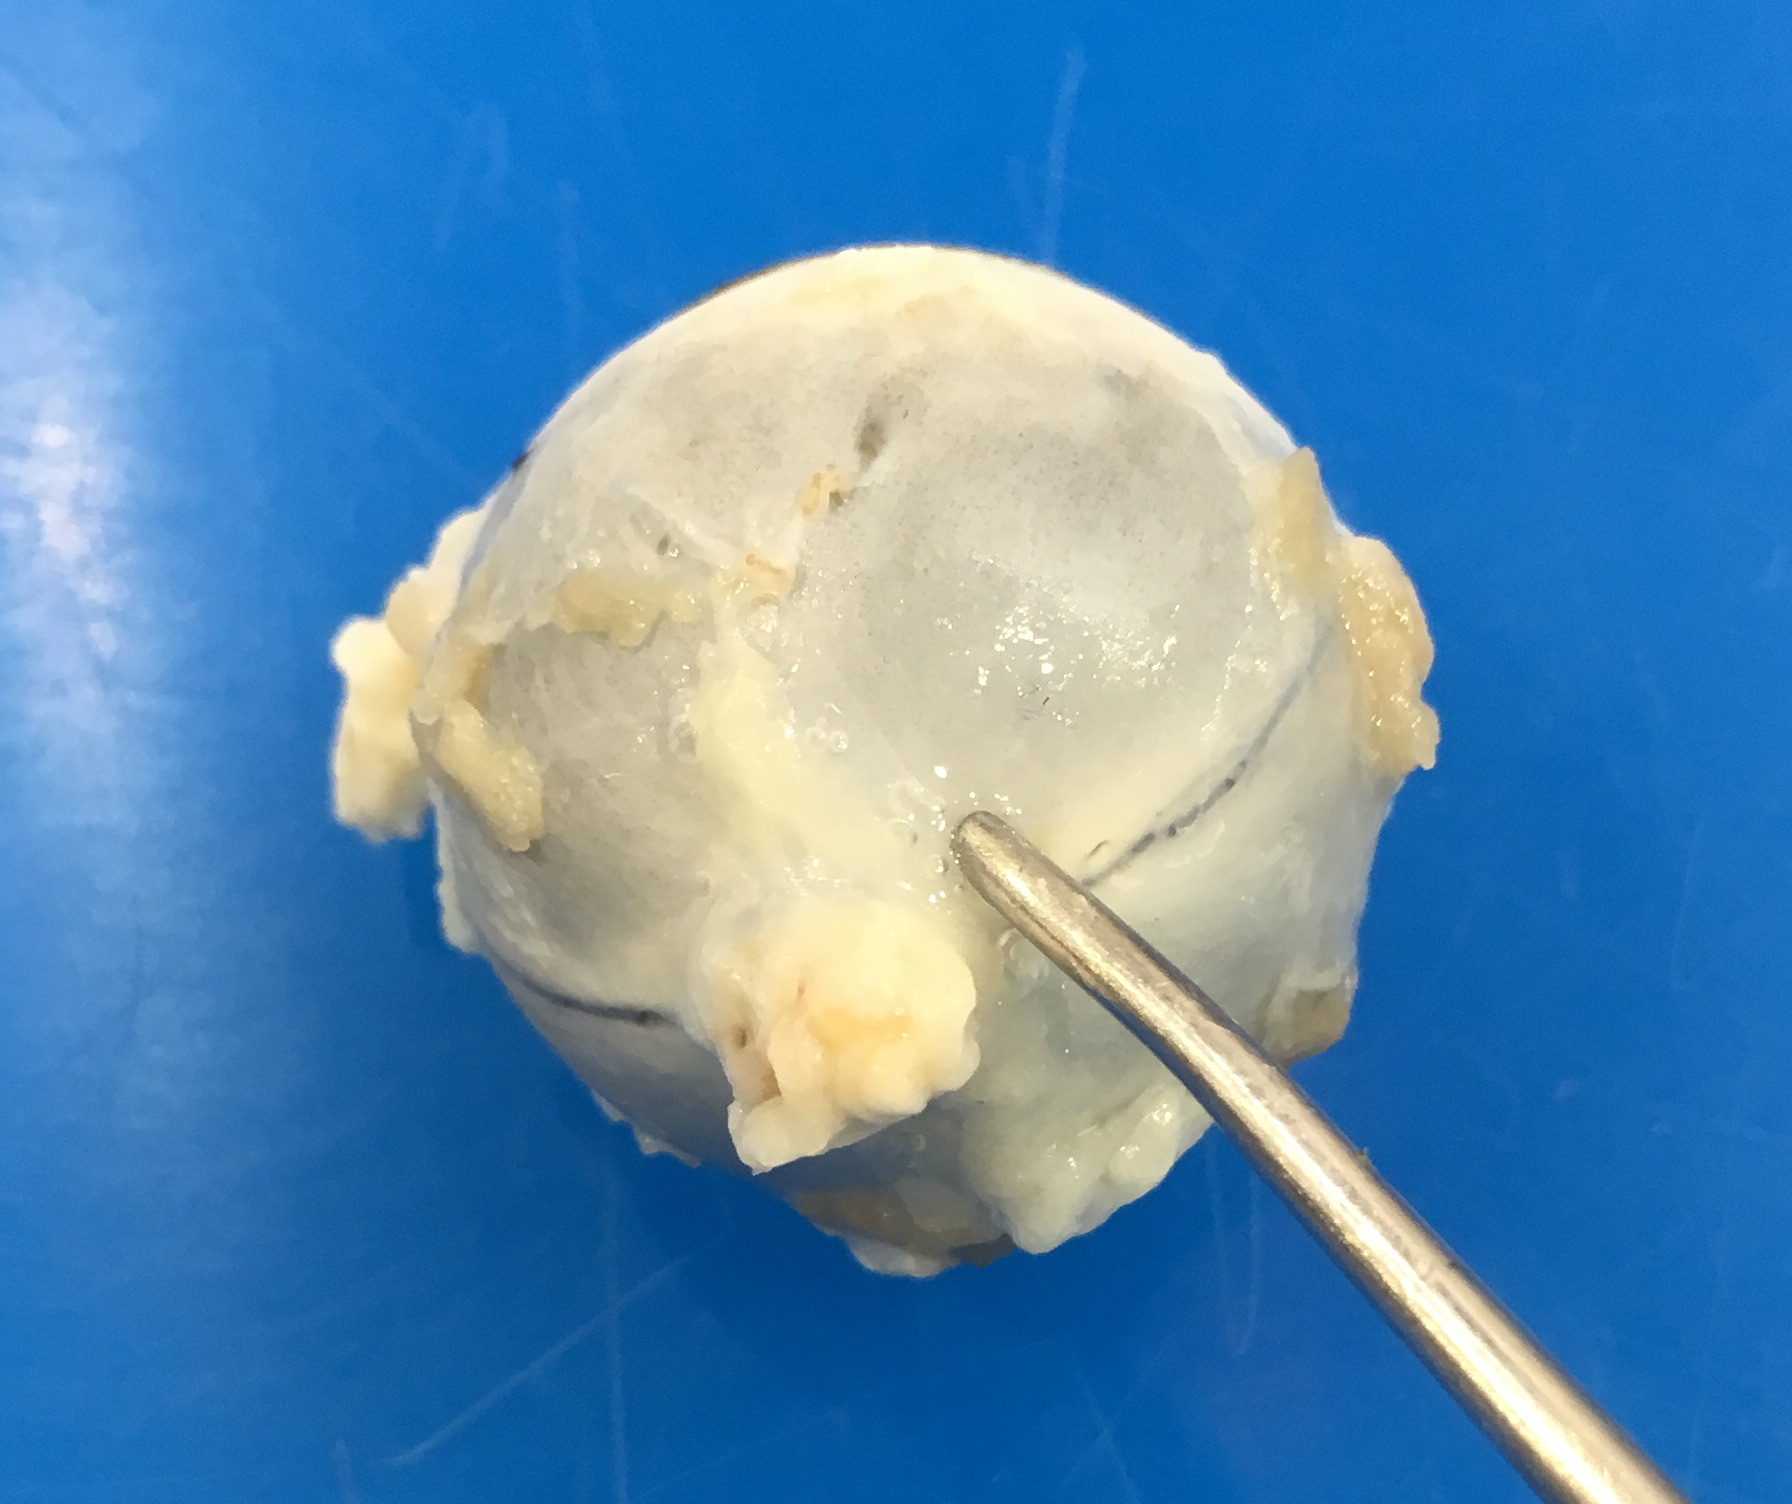
\includegraphics[width=0.6\linewidth]{images/globe-biopsy} 

}

\caption{Landmarks for injecting the globe with formalin. The eye is oriented as it would be in a live patient. The probe (representing an ideal location to inject formalin) is at the caudal aspect of the eye, and just slightly dorsal.}\label{fig:globe-biopsy}
\end{figure}

Always remember to \textbf{include a detailed and succinct history}.
Many of the eyes that are submitted for pathology are at a similar
``end-stage'', and determining the underlying etiology is often
impossible based on histopathology alone. The more information you
provide, the more information the pathologist can then provide back to
you. Don't forget to include the duration of the clinical signs,
treatments administered, and your differential diagnoses.

\section{Pathology of the conjunctiva and
eyelids}\label{pathology-of-the-conjunctiva-and-eyelids}

\subsection{Conjunctivitis}\label{conjunctivitis}

A variety of different infectious agents can lead to inflammation of the
conjunctiva. Among the most important in a variety of species is
\emph{Chlamydophila}. In particular, in the cat, \emph{C. felis} is
often associated with a primary conjunctivitis, presenting with mucoid
neutrophilic ocular discharge. The condition is dealt with clinically
and these globes are rarely progress to the point where they are
examined microscopically. Occasionally, conjunctival biopsies may be
evaluated.

\subsection{Dermoid}\label{dermoid}

Dermoids are a form of choristoma: the formation of a normal structure
in an abnormal place. In the case of a conjunctival (or corneal)
dermoid, there is a nodule of skin present, which may be haired (Figure
\ref{fig:dermoid}). These lesions are dramatic and odd, but are usually
corrected through a keratectomy.

\begin{figure}

{\centering 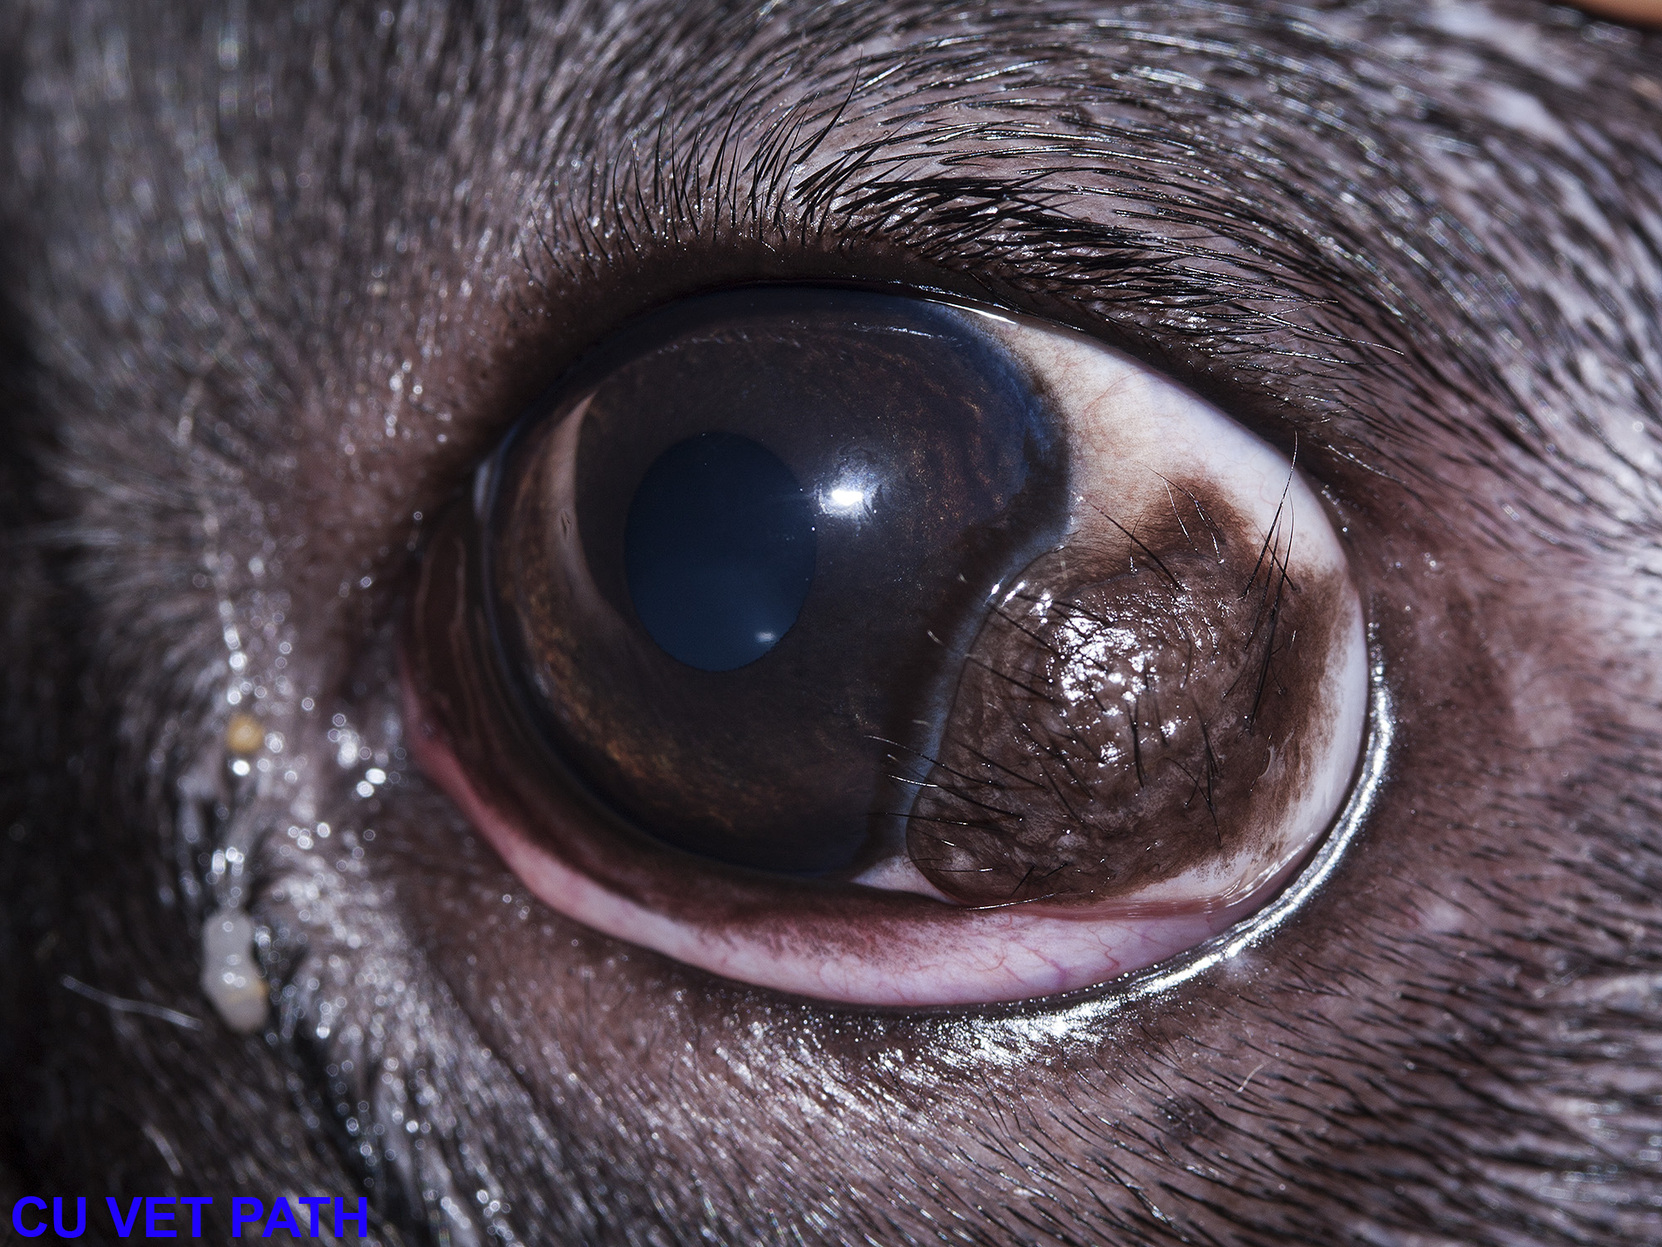
\includegraphics{images/dermoid_F33854} 

}

\caption{A dermoid present at the limbus (Image F33854 from Noah's Arkive)}\label{fig:dermoid}
\end{figure}

\subsection{Meibomian gland adenoma}\label{meibomian-gland-adenoma}

These are common neoplasms that occur at the eyelid margin, the only
place in the body in which Meibomian glands are found. They make up
almost 70 \% of canine eyelid neoplasms, and are therefore \textbf{the
most common eyelid neoplasm of the dog}. They are the eyelid equivalent
to a cutaneous sebaceous adenoma, and are similarly benign and cured
with complete resection. Grossly, they are usually well circumscribed
and multilobular. Leakage of gland contents frequently creates a local
granulomatous reaction that accompanies the neoplasm, known as a
\textbf{chalazion}.

\hypertarget{conjunctival-squamous-cell-carcinoma}{\subsection{Conjunctival
squamous cell carcinoma}\label{conjunctival-squamous-cell-carcinoma}}

Squamous cell carcinomas (SCC) of the conjunctiva or eyelid occur in all
species, but are most common and most important in the horse and cow. In
fact, SCC and
\protect\hyperlink{infectious-bovine-keratoconjunctivitis}{Infectious
bovine keratoconjunctivitis} are the two most important ocular
conditions of cattle. In both horses and cattle, UV light is thought to
play a role in the pathogenesis, and those breeds with poorly pigmented
skin are at increased risk. These neoplasms are infiltrative and have
metastatic potential, though the true metastatic risk is poorly
documented, and likely occurs late in disease. There is however a strong
possibility that an animal may develop multiple conjunctival SCCs, and
whether these separate masses are related is uncertain.

Grossly, conjunctival SCCs are typically raised, tan, and nodular. They
are frequently ulcerated, with superifical crusts and hemorrhage. In
cattle, they most frequently arise on the bulbar conjunctiva at the
limbus, whereas the third eyelid is the most frequently affected in
horses. In cats, SCC tends to arise from the skin of the eyelid. For
unknown reasons, dogs seem relatively spared from developing SCCs.

\subsection{Melanocytic tumours}\label{melanocytic-tumours}

Melanomas are frequent tumours of the eyelids and conjunctiva, and, in
dogs, \textbf{prognosis mostly depends on location}. Melanocytic tumours
arising at the eyelid margin are benign (like a dermal melanocytoma).
Those that arise from the conjunctiva are more invasive and prone to
recurrence (somewhat like oral melanomas). Those that arise from the
limbus are benign.

\hypertarget{entropion-and-ectropion}{\subsection{Entropion and
ectropion}\label{entropion-and-ectropion}}

Entropion refers to the inward folding of the eyelid, and is most common
on the upper eyelid. Ectropion refers to an eyelid that turns slightly
outward, and is more common in the lower eyelid. These are primarily
clinical conditions and the underlying pathology is unremarkable. Both
are most commonly seen in dogs, and there are strong breed
predilections. Due to mechanical abraision, entropion may result in
physical damage to the cornea. The condition is seen routinely and is
easily fixed with minor surgery.

\section{Pathology of the cornea}\label{pathology-of-the-cornea}

\subsection{Corneal ulcers}\label{corneal-ulcers}

Corneal ulcers - the erosion of the surface epithelium with exposure of
the underlying corneal stroma - are \textbf{extremely common} and occur
for a variety of reasons. A few specific etiologies are dealt with
below, however, there are some generalities that can be applied to most
corneal ulcers, regardless of cause.

Recall that the corneal stroma is \emph{kept in a dehydrated state}:
this is accomplished by having an impermeable epithelial surface, as
well as active pumps along the corneal endothelium (explained further
\protect\hyperlink{ocular-anatomy}{Ocular anatomy}). Thus, any break to
the epithelial barrier will result in \textbf{stromal edema} -- through
the absorption of tear film -- that manifests clinically as a blue-ish
tinged cloudiness of the cornea. Neutrophils found in the tear film can
also enter the stroma through the disrupted barrier.

What happens next is dependent on the degree of corneal injury. If the
injury is relatively minor -- for example, the erosion of the
superficial epithelium and perhaps a small amount of the stroma -- then
the remaining epithelium can slide over the defect, providing an
initial, thin barrier. Mitosis begins within 24 hours so that the
epithelium will soon return to its normal thickness. Be aware, however,
that for healing to be succesful, \textbf{the epithelium must be able to
adhere to the underlying stroma}. Some cases of refractory corneal
ulcers occur due to the presence of degenerative superficial stroma that
fails to provide an adequate foundation onto which the epithelium can
anchor. Procedures that remove the uncooperative tissue (e.g.~grid
keratectomy) allow new granulation to form, thereby providing a scaffold
for the epithelium to anchor to.

Deeper wounds -- those with more than 1/3 of the stroma affected, give
or take -- require a bit more investment in healing. Epithelial sliding
cannot occur in these cases before the stroma is rebuilt. To rebuild
corneal stroma, the keratocytes (fibrocytes of the corneal stroma)
undergo fibroblastic differentiation and begin producing ground
substance. Fibroblasts and small blood vessels also begin migrating from
the limbus, and it is these fibroblasts that are the primary source of
collagen. This migration takes time. Approximatley 4 days to get
started, then about 1 mm every day thereafter. The new cornea is never
quite the same as the original. Over time, the newly deposited collagen
will organize to resemble normal stroma, and the tissue will become less
cellular, a scar will be detectable. The degree to which a scar affects
vision is dependent on the initial insult (Fun fact: I have a scar
across my cornea, courtesy of an errant hockey stick. It doesn't
obstruct my vision at all). The epithelial component of a larger wound
is also different: in large defects, epithelial reserve cells from the
limbus are recruited, and these cells have a conjunctival, rather than
corneal, phenotype, and may be pigmented, though if the injurius
stimulus is removed, these epithelial cells will gradually become more
``corneal''.

Ulcers that progress may erode through the entire corneal stroma all the
way to Descemet's membrane. In these cases, Descemet's membrane may
protrude through the corneal defect, creating a small structure known as
a Descemetocele. \textbf{These cases are clinical emergencies}, as the
membrane may rupture at any time, resulting in a full corneal rupture
with significant adverse consequences. A ruptured cornea will repair
with fibrin, but occasionally the iris may prolapse into the defect,
forming an anterior synechia - an irreversible change.

Further complicating matters is whether the injury is sterile or
infected. Sterile injuries tend to heal more quickly, while those that
are complicated by infectious agents recruit more neutrophils, which
induce bystander damage by lysing the corneal stroma (keratomalacia),
and may delay healing, or even worse, lead to rapidly progressing
corneal damage in the form of a melting ulcer.

\subsection{Keratoconjunctivitis
sicca}\label{keratoconjunctivitis-sicca}

Keratoconjunctivitis sicca (KCS) is a condition in which the cornea
desiccates (dries out), usually due to a decreased \textbf{quantity} of
tear film, and rarely due to an altered quality of tear. The condition
is most common in dogs, in which it is progressive and chronic. The
etiology is unknown, but the success of immunosuppressive therapy
suggests an \textbf{autoimmune basis}.

The lesions depend on the degree to which tear film production is
affected. Most cases are moderate in onset, and result in chronic injury
to the cornea, manifesting as cutaneous metaplasia. As tear film
decreases, injury becomes more severe, and corneal ulcers may develop.
There is nothing distinctive about these ulcers, with the sole exception
that corneal edema may be minimal (as there is no tear film providing
water to the cornea).

The condition is readily treated with artificial tears and
immunosuppressive therapy.

\subsection{Fungal keratitis}\label{fungal-keratitis}

Fungal keratitis is a particularly common and important issue in horses.
\textbf{It is usually iatrogenic}, resulting from the treatment of a
routine corneal ulcer with antibiotics, and especially corticosteroids.
Colonization of the wound by fungi (usually \emph{Aspergillus}) results
in a deep ulcerative keratitis and is accompanied by suppurative
keratomalacia that is refractory to treatment with antibiotics. For
unknown reasons, the fungi are often found deep in the cornea near
Descemet's membrane. This unusual distribution explains why superficial
sampling -- either corneal scrapes or corneal biopsy -- may miss the
fungi, and produce false-negative results. Do not be surprised,
therefore, when a pathology report from a horse with suspected fungal
keratitis informs you that although no organisms were seen, the
condition cannot be ruled out!

\subsection{Herpesviral keratitis}\label{herpesviral-keratitis}

Feline herpesvirus 1 can cause a keratitis or keratoconjunctivitis.
Clinical signs are typically a mucopurulent ocular discharge with
conjunctivitis and keratitis (and rhinotracheitis). In younger cats, the
disease typically manifests as conjunctivitis without keratitis, whereas
in adult cats the opposite is true. In adults, the corneal lesions may
present as shallow erosions that appear as very small, multifocal
erosions or ulcers that may coalesce and have a branching ``dendritic''"
appearance (Figure \ref{fig:dendritic}). Alternatively, in severe cases
usually associated with immunosuppression, a severe keratitis may
develop, with notable corneal edema and corneal vascularization.

\begin{figure}

{\centering 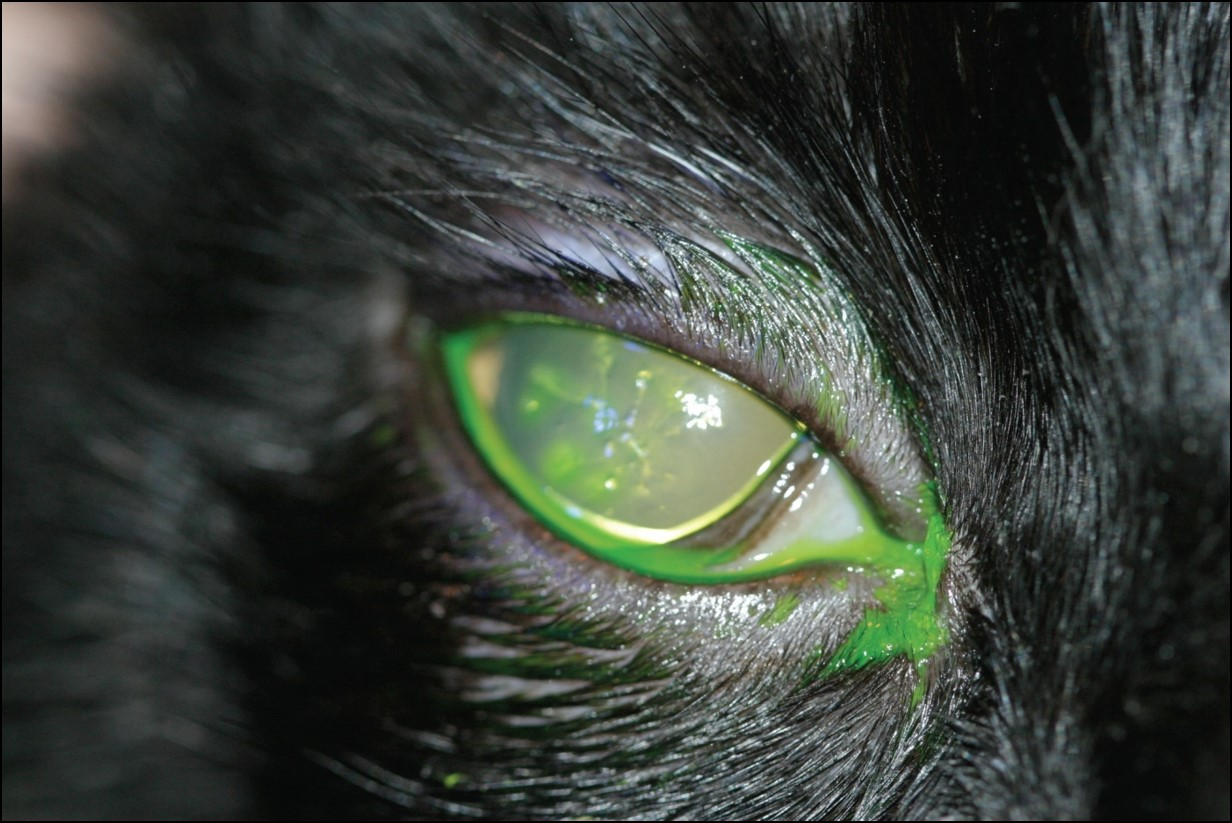
\includegraphics{images/dendritic_ulcer_feline} 

}

\caption{Herpetic keratitis with dendritic (branching) ulcers. Image from [Sandmeyer et al, 2010](https://www.ncbi.nlm.nih.gov/pmc/articles/PMC2885128/)}\label{fig:dendritic}
\end{figure}

\hypertarget{infectious-bovine-keratoconjunctivitis}{\subsection{Infectious
bovine
keratoconjunctivitis}\label{infectious-bovine-keratoconjunctivitis}}

Infectious bovine keratoconjunctivitis, also called ``pinkeye'', is
caused by \emph{Moraxella bovis}. \textbf{Along with
\protect\hyperlink{conjunctival-squamous-cell-carcinoma}{Conjunctival
squamous cell carcinoma}, it is the most important ocular condition of
cattle.}

Cattle are infected by \emph{Moraxella bovis} via fly vectors, and thus
the disease is more common during the summer months. Upon infection, the
bacteria adhere and then invade into the corneal epithelium, resulting
in a small corneal ulcer accompanied by corneal edema and hyperemia. If
left untreated, the ulcer will enlarge, deepen, and become infiltrated
by large numbers of neutrophils. Damage from the indiscriminate
neutrophils results in keratomalacia. In most cases, healing occurs as
the necrotic cornea is shed and granulation tissue fills the wound,
eventually scarring over. Despite the often relatively large ulcer found
in the acute stages of the condition, the final scar is often small and
clinically insignificant.

\subsection{Dystrophies and
depositions}\label{dystrophies-and-depositions}

The accumulation of material within the cornea is relatively frequently
seen in clinical practice. It may occur as dystrophies or deposits.

A dystrophy is an inherited, bilateral, defect in structure or function
of one of the components of the cornea. It is not triggered by injury or
disease, either directly to the eye or elsewhere in the body. The most
common, which are seen in dogs, are lipid and crystalline dystrophies.
In the case of the former, cholesterol is deposited in the corneal
stroma, while in the later mineralization may be present in the
superficial corneal stroma.

Corneal deposits typically occur secondarily to metabolic disease or
injury. Metabolic deposits include mineral, lipid, or pigment. The most
common metabolic deposit, again seen in dogs, takes the form of corneal
lipid associated with hyperlipidemia of any cause - though often
associated with Cushing's disease, diabetes mellitus, or hypothyroidism.

Corneal deposits secondary to injury are again most common in dogs.
Melanin deposits occur in corneas subject to chronic irritation.

\section{Pathology of the uvea}\label{pathology-of-the-uvea}

Uveitis is commonly encountered, and a good understanding of
pathophysiology of the disease will serve you well in practice.
Unfortunately, like many other parts of ophthalmology, the terms related
to uveitis are confusing, and I suggest you review and then keep the
\protect\hyperlink{glossary}{Glossary} handy while going through this
section.

The uvea represents three structures that compose the vascular supply to
the eye: the iris, ciliary body, and choroid (see Figure \ref{fig:globe}
to refresh your memory). Inflammation of the uveal structures --
especially inflammation that is on-going or recurrent -- can have a wide
range of impacts beyond the uvea itself.

The iris is a relatively porous tissue, and when inflamed, leukocytes,
blood and/or fibrin exit vessels and rapidly transit through the iris
and into the aqueous. Clinically (or grossly), this manifests as an
accumulation of cells and/or protein in the anterior chamber. Hyphema is
the presence of hemorrhage within the anterior chamber, while hypopyon
is an accumulation of neutrophils. Aqueous flare is the clinically
visualized presence of increased protein in the aqueous humour.

Corneal edema is a reasonably common clinically observed secondary
effect of uveitis. It can result from damage to the corneal endothelium,
or from a cytokine-mediated increase in vascular permeability in the
peripheral limbic vessels.

Fibrin within the anterior chamber may coat the iris, and lead to
adherence of the iris to the cornea (anterior synechia) or to the lens
(posterior synechia).

A common sequela of inflammation is the development of granulation
tissue, and the eye is no exception. In the eye, granulation tissue
often forms as a membrane that layers pre-existing ocular structures.
Unfortunately for vision, the delicate and carefully organized
structures of the eye are frequently altered by these membranes of
granulation tissue. The exact consequence of the membrane depends on the
location in which it forms: a pre-iridal fibrovascular membrane, for
example, forms on the surface of the iris and may a) grow over the
iridocorneal angle, leading to glaucoma (see the section on
\protect\hyperlink{glaucoma}{Glaucoma} for more details); or it may b)
grow over the pupil, leading to complete pupillary block and iris bombe;
or it may c) simply cover the iris, and following maturation and
contraction, deviate the free edge of the iris forward, leading to
ectropion uvea. Alternatively, a membrane developing in the posterior
segment over the choroid, known as a cyclitic membrane, may lead to
retinal detachment as it matures and contracts (known as tractional
retinal detachment).

The lens, too, is susceptible to the secondary effects of uveitis.
Cataracts may develop, possibly a result of uveal attachment to its
surface (posterior synechia), or an alteration in aqueous flow, or
simply by an excess of inflammatory cytokines and by-products appearing
in the aqueous. More information can be found in the section on the
\protect\hyperlink{pathology-of-the-lens}{Pathology of the lens}.

There are many causes of uveitis, including a number of infectious
organisms that we are not going to cover. Below are some of the more
commonly encountered conditions.

\subsection{Mycotic endophthalmitis}\label{mycotic-endophthalmitis}

A variety of different fungal organisms can gain access to the eye.
\emph{Blastomyces dermatitis} is the most frequent in dogs, while
\emph{Cryptococcus neoformans} is the most common in cats. There is
nothing particularly surprising about these agents: they present with a
profound, usually pyogranulomatous endophthalmitis that one would expect
following a fungal infection. Retinal detachment may result secondary to
the accumulation of inflammatory exudates.

\subsection{Uveodermatologic syndrome (Vogt-Koyanagi-Harada-like
syndrome)}\label{uveodermatologic-syndrome-vogt-koyanagi-harada-like-syndrome}

This syndrome is relatively frequently seen in dogs, particularly in
arctic-type breeds (Siberian huskies, Alaskan malamutes, Akitas, etc).
The root of the condition is an immune-mediated targeting of proteins
involved in the production of melanin. The inflammation, \textbf{which
is granulomatous in nature}, targets the uvea and the skin of the face,
though the ocular disease is typically more severe and of more
consequence.

Because the inflammation targets the production of melanin, \textbf{one
of the most notable clinical signs is uveal and dermal depigmentation}.
The granulomatous inflammation of the uvea leads to destruction of
melanocytes and dispersal of melanin. Inflammation in the choroid tends
to be most severe, and can lead to
\protect\hyperlink{retinal-detachment}{Retinal detachment},
\protect\hyperlink{pre-iridial-fibrovascular-membranes-pifm}{PIFM}, and
\protect\hyperlink{glaucoma}{glaucoma.}

\subsection{Canine adenovirus}\label{canine-adenovirus}

In North America, canine adenovirus is mostly of historical relevance
due to widespread vaccination. In areas with poor vaccination, the
ocular manifestation of adenovirus is still significant.

In unvaccinated animals -- or, rarely, animals receiving a modified live
virus -- canine adenovirus infects the uveal and corneal endothelial
cells. Damage to uveal endothelium can lead to anterior uveitis, while
corneal edema (due to damage to the corneal endothelium) may develop.

\hypertarget{equine-recurrent-uveitis}{\subsection{Equine recurrent
uveitis}\label{equine-recurrent-uveitis}}

Equine recurrent uveitis (ERU) is \textbf{the most common cause of
glaucoma, cataracts, and blindness in horses}. Although the condition
may start out affecting only one eye, it virtually always ends up being
bilateral. As it's name suggests, the disease presents as waxing and
waning episodes of uveitis that gradually increase in frequency. The
gross/clinical signs of the disease are, like many ocular diseases, a
constellation of lesions that require an astute ophthalmological exam.
Uveitis, of course, is one of the main features, manifesting as
increased proteinaceous content in the anterior chamber (``aqueous
flare'') and vitreous. Corneal edema is also frequently present. In
severe cases, there may be hyphema or hypopyon. In more chronic cases,
cataracts, lens luxation, retinal detachment, and glaucoma may all be
observed.

Microscopically in the early course of disease, there tends to be
neutrophilic inflammation of the iris and ciliary body with fibrin and
proteinaceous material found within the anterior chamber. Over a fairly
short period of time, the inflammation becomes predominantly
lymphoplasmacytic and histiocytic. In the chronic stages,
lymphoplasmacytic inflammation of the entire uvea (panuveitis)
dominates, and lymphoid follicles within the iris and ciliary body are
characteristic.

The pathogenesis of ERU is still under investigation and is not fully
understood. The current favoured theory is that \textbf{ERU represents a
multifactorial immune-mediated disease}. There is a body of evidence --
that is \emph{not} conclusive -- that implicates previous exposure or
infection to \emph{Leptospira interrogans} serovar \emph{pomona} as an
initiating cause. Many cases have been associated with seropositivity
for \emph{Leptospira}, and experimental infection can induce the
disease; however, \textbf{a significant portion of cases are not
associated with leptospirosis}, rendering this hypothesis somewhat
flawed. Instead, the modern belief is that some initiating cause -- at
this point, unknown -- causes a uveitis that \emph{alters the normal
immune privilege status of the eye}. Proteins within the eye that were
previously restricted may become accessible to the immune system, and
become antigenic stimuli as a result; similarly, antibodies generated
through exposure to exogenous sources that may cross-react with ocular
antigens may now have access to ocular structures. This breakdown in
ocular immune privilege is what may lead to the continuing inflammation
within the eye, and regardless of the initial cause, is probably the
more important aspect of the disease.

\hypertarget{feline-lymphonodular-uveitis}{\subsection{Feline
lymphonodular uveitis}\label{feline-lymphonodular-uveitis}}

Feline lymphonodular uveitis, also known as feline lymphoplasmacytic
uveitis, is the most common cause of uveitis in the cat, and along with
\protect\hyperlink{diffuse-iris-melanoma}{Diffuse iris melanoma}, is one
of the top causes of feline glaucoma. The condition generally starts off
unilaterally, however, the contralateral eye is to be considered at
risk.

Cats with the condition may present with one or more of the following
symptoms: corneal edema with neovascularization; keratitic precipitates
(cellular deposits on the corneal endothelium); and/or thickened irides.
Eventually, glaucoma may develop, though the mechanism through which
this occurs is unknown. Microscopically, the disease is characterized
(as expected) by lymphoplasmacytic inflammation of the uvea,
particularly within the iris, where lymphoid nodules may develop in
severe cases.

The cause of feline lymphondular uveitis is unknown, but the
pathogenesis is thought to be similar to
\protect\hyperlink{equine-recurrent-uveitis}{ERU}.

\subsection{Feline infectious
peritonitis}\label{feline-infectious-peritonitis}

As with other locations in the body, feline infectious peritonitis virus
can causes a significant vasculitis within the vascular structures of
the eye (i.e.~the uvea). Pyogranulomatous inflammation, particularly of
the anterior uvea, tends to predominate. Grossly, anterior uveitis,
manifesting as aqueous flare, is common. Diagnosis cannot be made on
histopathology alone; ancillary diagnostics (e.g.~IHC) are required.

\subsection{Bovine MCF-associated
uveitis}\label{bovine-mcf-associated-uveitis}

Malignant catarrhal fever virus causes a vasculitis with invasion of the
vascular wall by lymphocytes. It is therefore a lymphocytic uveitis.
Uveitis and corneal edema are noted grossly, and, when considered with
the other gross lesions of MCF, the corneal edema can be particularly
useful in helping distinguish between MCF and other mucosal diseases.

\subsection{Lens-induced uveitis}\label{lens-induced-uveitis}

(Please refer to the section on the
\protect\hyperlink{pathology-of-the-lens}{lens} for more information on
the lens itself).

The lens is an immunologically privileged site, and the proteins that
make up the lens fibers are thus not-recognized as self. Exposure of
these proteins to the immune system can therefore elicit an immune
response, the severity of which depends to some degree on the amount of
protein encountered.

\subsubsection{Phacolytic uveitis}\label{phacolytic-uveitis}

Phacolytic uveitis refers to a mild to moderate lymphoplasmacytic
uveitis resulting from the \textbf{leakage of liquefied lens protein
through an intact lens capsule}. Liquefaction of lens proteins occurs
routinely as cataracts mature; it can be relatively safely assumed that
all animals with mature cataract have at least some degree of phacolytic
uveitis. This condition cannot be distinguished from other idiopathic
anterior uveitis based on histopathology (see
\protect\hyperlink{equine-recurrent-uveitis}{Equine recurrent uveitis}
and \protect\hyperlink{feline-lymphonodular-uveitis}{Feline
lymphonodular uveitis}.

\subsubsection{Phacoclastic uveitis}\label{phacoclastic-uveitis}

In contrast to the relatively mild inflammatory response in a phacolytic
uveitis, the inflammation in phacoclastic uveitis is severe, profound,
and centered around a \textbf{lens material extruded through a ruptured
lens capsule}. Rupture of the lens capsule is most often caused by a
penetrating foreign object (e.g.~a thorn, or, more frequently, the
business end of a cat's paw). The type of inflammation is somewhat
variable, but in the acute stages is neutrophilic and accompanied by
fibrin; in more chronic cases, fibrosis with little inflammation
dominates.

Iatrogenic phacoclastic uveitis may occur during cataract surgery, if
lens protein is inadvertently left behind.

In rabbits, infection with \emph{Encephalitozoon cuniculi} can lead to a
phacoclastic uveitis, presumably through infection derived weakening of
the lens capsule. The inflammation is characteristically granulomatous.

\hypertarget{diffuse-iris-melanoma}{\subsection{Diffuse iris
melanoma}\label{diffuse-iris-melanoma}}

\textbf{This is an important (and contentious!) condition seen in cats}.
It is the most common ocular neoplasm of cats. The condition begins as
patchy areas of golden brown pigmentation on the anterior surface iris,
which progress slowly (over the course of years) to coalesce and
gradually expand the iris. The pupil may become irregular. Expansion and
invasion into adjacent structures eventually leads to
\protect\hyperlink{glaucoma}{Glaucoma} in virtually all cases, but this
eventual fate \textbf{may take years to occur}. Feline diffuse iris
melanomas also have significant metastatic potential. Seeding of the
aqueous by neoplastic cells gives them access to outflow and general
circulation. The neoplasm may then grow in the lungs, liver, and/or
lymph nodes. There is considerable debate regarding the literature and
studies on prognosis of cats with diffuse iris melanoma. Some advocate
swift enucleation following a diagnosis, arguing that this reduces
opportunity for metastasis and thus complications. Others suggest that
the metastatic potential is relatively low, and that systemic disease
resulting from said metastases is not a guarantee, and thus recommend
waiting until complications (i.e.
\protect\hyperlink{glaucoma}{Glaucoma}) have occurred prior to
enucleation.

\hypertarget{canine-anterior-uvea-melanocytoma}{\subsection{Canine
anterior uvea melanocytoma}\label{canine-anterior-uvea-melanocytoma}}

\textbf{This is the most frequent ocular tumour of dogs}. It presents as
an expansile mass originating from the root of the iris that is usually
pigmented. Prognosis based on clinical/gross appearance is challenging:
a small proportion (\textasciitilde{} 5\%) are malignant and have true
metastatic potential, but this determination is based on histopathology,
and cannot be predicted without a biopsy. However, even those that are
histologically benign may represent a significant problem for the globe,
as most will grow to occlude the ciliary cleft, leading to
\protect\hyperlink{glaucoma}{Glaucoma}.

\hypertarget{pathology-of-the-lens}{\section{Pathology of the
lens}\label{pathology-of-the-lens}}

The lens is a disc-like structure suspended by zonules at the posterior
aspect of the anterior segment. It is avascular, and relies completely
on the diffusion of nutrients from the aqueous humour. It's deceptively
simple appearance belies it's important function: the refraction of
light onto the retina to provide focus.

The lens is a living tissue, albeit a relatively simple one (See Figure
\ref{fig:lens}). It is enclosed by the lens capsule, which is the
basement membrane of the lens epithelial cells that make up the body of
the lens. The capsule is \emph{impermeable to large proteins, but allows
the entry of water and other nutrients, making the lens an
immunologically privileged site}. The lens epithelium lines the anterior
half (and \emph{only} the anterior half) of the lens capsule in a
single, cuboidal layer. The lens epithelium is mitotically active, and
continually divides to produce additional epithelial cells. These cells
migrate centrally and elongate, forming the long fibers that make up the
lens. As the epithelial cells differentiate, they lose their nuclei and
organelles, forming the clear structure important to its function. Like
the cornea, the lens maintains itself in a dehydrated state to help
maintain its clarity; this is mediated by an active Na-K pump located on
the anterior lens epithelial cells.

\begin{figure}

{\centering 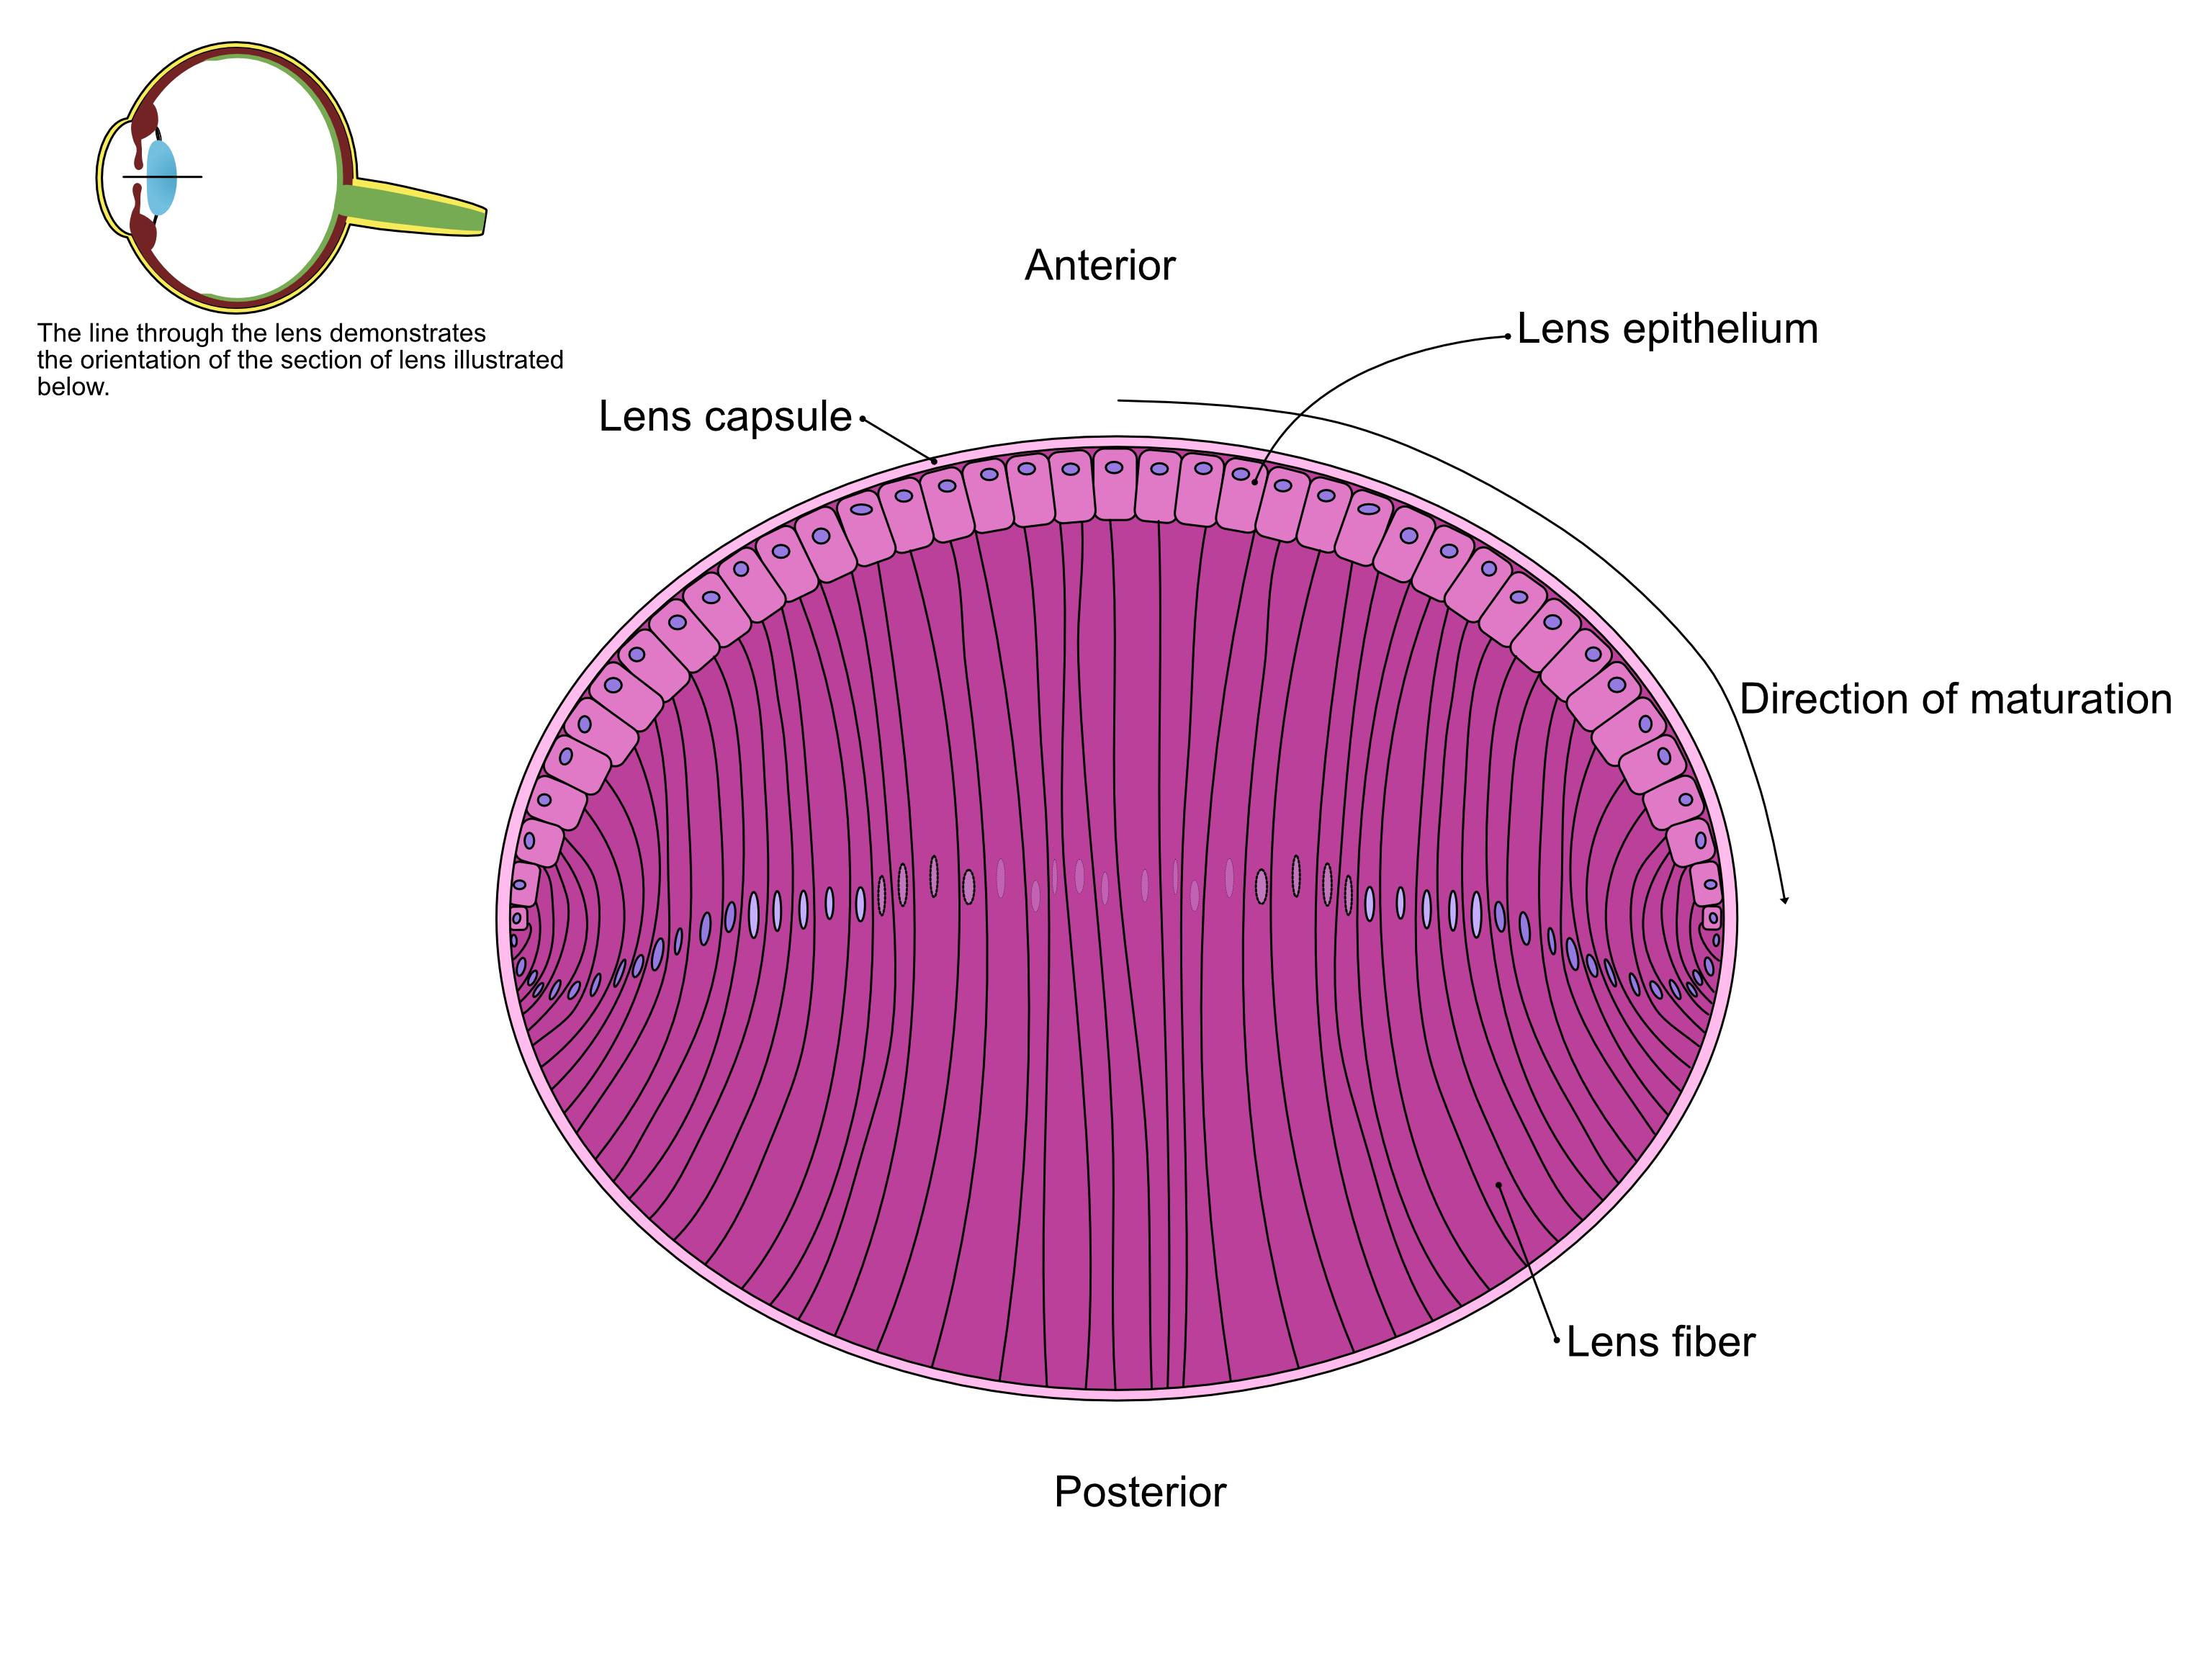
\includegraphics[width=0.6\linewidth]{images/lens3x} 

}

\caption{An anterior-posterior illustration of the lens, demonstrating the anterior epithelium, nuclear bow, lens capsule, and lens fibers.}\label{fig:lens}
\end{figure}

The lens survives mainly on glucose delivered by the aqueous humour,
which is metabolized via anaerobic glycolysis and the hexokinase pathway
to produce energy. This small piece of information is a \emph{critical
component to the understanding of the pathophysiology of cataracts}.

\subsection{Cataract}\label{cataract}

A cataract is defined as opacification of the lens. When severe, it is
readily diagnosed on histopathology, however, ophthalmological exam is a
\emph{far more sensitive and accurate method of diagnosing and
describing cataracts}.

The opacification of the lens is the result of alteration of the
normally dehydrated lens and its well-organized lens fibers. In response
to injury, the lens epithelium may attempt to proliferate, while lens
fibers frequently undergo degenerative and hydropic changes.
Proliferating epithelial cells may migrate to the normally acellular
posterior aspect of the lens, contributing to opacity. The epithelial
cells may also become hyperplastic along the anterior edge, and in some
cases, may undergo fibrous metaplasia and produce collagen. Hydropic
degeneration of epithelial cells may result in large, rounded cells
known as bladder cells. Existing lens fibers may liquefy and fragment,
forming characteristic globules of denatured lens proteins known as
Morgagnian globules.

With their superior ability to visualize and evaluate cataracts,
ophthalmologists are also able to classify cataracts in a variety of
different ways, including age of onset (e.g.~juvenile vs senile),
anatomic location (e.g.~subcapsular vs.~equatorial), extent (mature
vs.~hypermature), or pathogenesis. Because this is a course in
pathology, and not ophthalmology, we will focus primarily on classifying
cataracts according to their pathophysiology, rather than through other
metrics.

\subsubsection{Inherited}\label{inherited}

Inherited cataracts are most commonly reported in dogs, and are
relatively infrequent in other species. They may be congenital or may
appear at any stage in the life of the animal. Diagnosis of an inherited
cataract is based on the signalment, paying particular attention to
breed predispositions, the age of presentation, and the ophthalmologic
type of cataract. Histopathology alone \emph{cannot} distinguish between
types of cataracts.

\subsubsection{Diabetic cataracts}\label{diabetic-cataracts}

Diabetic cataracts are one of the most frequently encountered type of
cataract seen by practitioners. \textbf{They are most common in dogs}.

The pathogenesis of diabetic cataracts relates to the metabolism of
glucose. As noted earlier, the lens absorbs glucose from the aqueous
humour, and, using the \textbf{anaerobic hexokinase pathway},
metabolizes glucose into energy. In diabetic dogs, the concentration of
glucose in the blood and aqueous is elevated, and excess glucose enters
the lens. The concentration of glucose overwhelms the hexokinase pathway
and is shunted into the aldose reductase pathway, which results in the
production of \textbf{sorbitol}. Sorbitol is too large to exit the lens,
and as it accumulates, it causes an increase in the osmotic pressure
within the lens, leading to influx of water. The end result is hydropic
rupture of lens fibers that manifests clinically as a cataract.

\emph{Microscopically, there is nothing distinctive about a diabetic
cataract}. The diagnosis is based on clinical signs, symptoms, diagnosis
of diabetes mellitus, and ophthalmologic type of cataract.

Interestingly, it is not solely an increase in intraocular glucose that
leads to cataract. It would appear that there are species differences in
the amounts of aldose reductase within the lens, and it is these
differences that are thought to contribute to the frequency of diabetic
cataracts in different species. For example, although diabetes mellitus
is relatively common in cats, diabetic cataracts are rare, because the
concentration of aldose reducates within their lens is low.

\subsubsection{Other causes of
cataracts}\label{other-causes-of-cataracts}

There are several other causes of cataracts. Nutritional cataracts are
best described in carnivores that have been fed milk replacer, but the
pathogenesis is unclear.

Radiation therapy is a well-known risk factor for the development of
cataracts. Cataracts may develop approximately 6-12 months post-therapy,
and the risk of development is dependent on the dose received during
treatment. The underlying pathogenesis relates to necrosis of the
equatorial germinal lens epithelial cells.

Infectious agents may also lead to cataracts. In cattle, infection with
bovine viral diarrhea virus (BVDV) \emph{in utero} is associated with
cataract development. In fish, infection with the fluke
\emph{Diplostomum spathaceum} leads to cataracts.

Finally, luxation of the lens may result in cataract through unknown
means, though it is thought that disruption of nutrition is the
underlying cause.

\subsection{Luxation}\label{luxation}

Lens luxation (dislocation) may be complete or partial (subluxation). It
is a gross or clinical diagnosis: sectioning of the globe for histologic
process typically disrupts the normal anatomic position of the lens. A
luxated lens may be found partially or completely within the anterior
chamber, or it may remain in the posterior chamber. Displacement of the
lens into the anterior chamber can disrupt and obstruct the flow of the
aqueous, resulting in glaucoma.

Lens luxation may be primary or secondary. Primary lens luxations occur
without any known trauma or ocular disease, and may be spontaneous or
the result of inherited defects in the zonules.

More common is secondary luxation, or those with a known cause, which
may include trauma, weakened zonules due to a greatly expanded
glaucomatous globe, or zonules weakened secondarily to uveitis. Note
that glaucoma can both cause and be the result of lens luxation, and
that it can be difficult to separate cause and effect when presented
with a one-time snapshot of the lesions.

\subsection{Feline post-traumatic ocular
sarcoma}\label{feline-post-traumatic-ocular-sarcoma}

Cats suffering trauma or damage to the lens may present months to years
later with a malignant and destructive intraocular neoplasm known as
feline post-traumatic ocular sarcoma. Cats typically present with a
refractory uveitis, cataract, and a history of ocular trauma. The
neoplasm is thought to arise from malignant transformation of the lens
epithelium, possibly mirroring the pathogenesis of
post-vaccinal/injection site sarcoma that is occasionally seen in cats.

Grossly, the neoplasm is grey to white and proliferative, often
compresses the lens. The mass expands and grows along the circumference
of the globe, and is ultimately invasive, frequently infiltrating into
the optic nerve or sclera.

\section{Pathology of the globe}\label{pathology-of-the-globe}

Although many ocular diseases in reality affect most portions of the
globe, in this section we will deal primarily with conditions that have
severe consequences to multiple anatomical structures of the eye. The
most important condition is glaucoma. The developmental abnormalities
discussed below are relatively uncommon, especially when compared to the
incidence of glaucoma, which is a \textbf{complex, common, and important
condition, and one that you should know thoroughly}.

\hypertarget{glaucoma}{\subsection{Glaucoma}\label{glaucoma}}

Glaucoma is a clinical diagnosis and is by defined by a sustained and
damaging increase in intraocular pressure (IOP). Glaucoma has many
etiologies, and the effects of increased IOP manifest in just about
every structure in the globe. With that in mind, \emph{the impact to the
retina and optic nerve are the most important}, as damage to these
structures leads to loss of vision and pain.

Glaucoma is most common in dogs, followed by cats and horses. It is the
leading cause of enucleation in both dogs and cats.

Intraocular pressure is a balance between the production and drainage of
aqueous humour. Aqueous humour is produced by the epithelial lining of
the ciliary body and flows into the posterior chamber, where it provides
the lens with nutrients and oxygen while removing waste products. From
the posterior chamber the aqueous humour flows through the pupil into
the anterior chamber, where it provides the same services to the corneal
endothelium and stroma. Having served its purpose, the aqueous humour
then drains through the trabecular meshwork at the \textbf{iridocorneal
angle}, located in the anterior chamber at the junction of the cornea
and iris. From there, the aqueous humour enters a venous plexus and is
returned to systemic circulation.

Although in theory, an increase in intraocular pressure could be due to
an increase in production or a decrease in outflow, \textbf{glaucoma is
\emph{never} due to increased production, and is always the result of
decreased outflow}.

The pathological changes to the eye caused by glaucoma can be related to
four basic pathophysiologic processes:

\begin{enumerate}
\def\labelenumi{\arabic{enumi}.}
\tightlist
\item
  Direct or indirect physical effects on cells caused by increased IOP.
\item
  Compression of vasculature from increased IOP leading to hypoxia.
\item
  Stagnation of the flow aqueous humour.
\item
  Autotoxicity.
\end{enumerate}

Let's consider each of the structures of the globe and how they may be
affected by each process, and what the consequences would be. Remember,
though, that it is the \textbf{damage to the retina and optic nerve that
leads to blindness in these patients}.

Globe:

\begin{itemize}
\tightlist
\item
  Increased IOP may lead to an enlarged globe that protrudes slightly
  from the orbit (buphthalmos). This change is dependent to a degree on
  the age and species of the animal; younger animals with more elastic
  collagen are more likely to experience a stretch in the sclera.
\end{itemize}

Cornea:

\begin{itemize}
\tightlist
\item
  A buphthalmic globe is susceptible to corneal desiccation and lack of
  proper protection from the eyelids. This can result in exposure
  keratitis leading to ulceration or epidermalization.
\item
  The corneal endothelium may be damaged by a) direct pressure; b) lack
  of proper aqueous flow (remember, the endothelium obtains nutrients,
  etc, from aqueous); and c) a stretched globe that results in a
  stretched and permeable endothelial barrier. These changes result in
  corneal edema.
\end{itemize}

Uvea:

\begin{itemize}
\tightlist
\item
  Pressure-induced hypoxia to the uvea can lead to atrophy of the uveal
  tissues, a change more commonly seen in chronic cases.
\item
  The damaged retina may release cytokines leading to a pre-iridial
  fibrovascular membrane.
\item
  Pressure-induced hypoxia to the vascular endothelium can lead to the
  leakage of proteins into the aqueous.
\end{itemize}

Lens:

\begin{itemize}
\tightlist
\item
  The decreased flow of aqueous humour can lead to cataract formation.
\item
  Buphthalmos may cause stretching and tearing of the zonular ligaments
  and luxation of the lens.
\end{itemize}

Retina:

\begin{itemize}
\tightlist
\item
  Damage to the retina is most profound on its inner most aspect,
  affecting the ganglion cells and the nerve fibers that carry sensory
  information from the retina to the optic nerve. In severe cases,
  atrophy can affect the entire retina (most often seen in dogs, see the
  section on \protect\hyperlink{pathology-of-the-retina}{retina} for
  more information).
\item
  Although an exact understanding of the pathophysiology of glaucomatous
  retinal atrophy is incomplete, certain elements are known: a)
  increased pressure on axons of ganglion cells interferes with axonal
  transport and contributes to ganglion cell degeneration; and b)
  severely increased IOP interferes with retinal blood supply, leading
  to ischemic injury.
\end{itemize}

Optic nerve:

\begin{itemize}
\tightlist
\item
  Cupping or bowing of the optic disc is characteristic and caused by
  increased IOP and/or decreased numbers of axons following ganglion
  cell death.

  \begin{itemize}
  \tightlist
  \item
    Cupping of the optic disc is a \emph{pathognomonic} lesion: in other
    words, it is a lesion found uniquely in glaucomatous globes.
  \end{itemize}
\end{itemize}

Unfortunately, the lesions of glaucoma rarely give us insight into the
underlying cause of increased IOP. The etiologies of glaucoma are many
and varied, and broadly can be divided into two categories: primary and
secondary glaucoma.

\subsubsection{Primary glaucoma}\label{primary-glaucoma}

Primary glaucomas arise \textbf{without significant acquired alteration
or disease to other structures of the globe}. Primary glaucomas can be
subdivided further into those which show maldevelopment of the
trabecular meshwork at the iridocorneal angle, a phenomenon known as
\textbf{goniodysgenesis}, and those which do not, typically referred to
as `open-angle glaucoma'.

Most dogs with primary glaucoma have goniodysgenesis. Goniodysgenesis is
present at birth and is thought to be inherited, yet glaucoma typically
only manifests in older dogs (5-12 years old). This finding, combined
with the fact that not all dogs with goniodysgenesis will develop
glaucoma, suggests that it is not the absence of the trabecular meshwork
itself that is the cause of glaucoma, but some other (less well
appreciated) alteration -- either physical, or, more likely, functional
-- that leads to increased IOP. Thus, \textbf{goniodysgenesis should be
regarded as a risk factor, but not a cause, for glaucoma}. A dog that
develops primary glaucoma and is observed to have goniodysgenesis is at
high risk for developing glaucoma in the other eye.

Primary open-angle glaucoma is uncommon, and is caused by dysfunctional
drainage at the iridocorneal angle, rather than abnormal iridocorneal
anatomy. It occurs in dogs, horses, and cats.

\subsubsection{Secondary glaucoma}\label{secondary-glaucoma}

Secondary glaucoma, as it's name would suggest, is diagnosed when
\textbf{acquired} changes to structures of the globe interfere with the
drainage of the aqueous humour. If you know and understand the path of
aqueous outflow, then it is possible, to some degree, to intuit some of
the changes that might impede the flow of the aqueous humor. Some
examples include, but are not limited to:

\begin{itemize}
\tightlist
\item
  Infiltration of the drainage angle by inflammatory cells or metastatic
  neoplastic disease
\item
  The development of a fibrous membrane that spans the iridocorneal
  angle
\item
  Adhesion between the pupil and the iris (posterior synechia)
\end{itemize}

\hypertarget{pre-iridial-fibrovascular-membranes-pifm}{\paragraph{Pre-iridial
fibrovascular membranes
(PIFM)}\label{pre-iridial-fibrovascular-membranes-pifm}}

Fibrovascular membranes develop when the concentration of angiogenic
factors in the vitreous and aqueous of the eye exceed normal levels. A
pre-iridal fibrovascular membrane (PIFM, pronounced ``piff-em'') is one
such membrane that develops on the anterior surface of the iris. Excess
angiogenic factors like VEGF are produced in a variety of conditions,
including corneal neovascularization (e.g.~from an ulcer), inflammation
(e.g.~chronic uveitis), neoplasia, and retinal hypoxia following
\protect\hyperlink{retinal-detachment}{retinal detachment.}

If a PIFM extends down the iris and across the pectinate ligament and
blocks the trabecular meshwork, thus obstructing the passage of aqueous
humor, secondary glaucoma is the result. Alternatively, PIFMs can grow
towards the lens, and can lead to an adhesion of the iris of the lens
(posterior synechia). If the adhesions spans the full 360 degrees of the
lens, it can obstruct the flow of aqueous from the posterior chamber,
resulting in pupillary block and forward bowing of the iris, known as
iris bombe (``bomb-ay''), and glaucoma.

\textbf{PIFMs are the most common cause of secondary glaucoma in the
dog}.

\paragraph{Cellular infiltration}\label{cellular-infiltration}

As is the case with the drain in a sink, small holes can be easily
plugged by debris, preventing adequate drainage. In the case of the eye,
the trabecular meshwork is particularly susceptible to becoming clogged
by cells, typically from neoplasia. Just like the sink, a clogged
trabecular meshwork does not drain properly, leading to accumulation of
aqueous humour and increased IOP.

In dogs, obstruction of the trabecular meshwork is most commonly
obstructed by neoplastic infiltrates, usually
\protect\hyperlink{canine-anterior-uvea-melanocytoma}{Canine anterior
uvea melanocytoma}.

In cats, \protect\hyperlink{diffuse-iris-melanoma}{Diffuse iris
melanoma} can directly obstruct the trabecular meshwork and lead to
glaucoma, and, along with
\protect\hyperlink{feline-lymphonodular-uveitis}{Feline lymphonodular
uveitis}, is the main cause of secondary glaucoma in this species.

\subsection{Developmental
abnormalities}\label{developmental-abnormalities}

True developmental abnormalities of the globe are rare. They include
anophthalmia, or complete absence of the eye (extremely rare and usually
bilateral); microphthalmia (a small, disorganized globe present within a
normal eye socket); and cyclopia (a single eye that failed to divide) or
synophthalmia (a single structure that contains duplicates of multiple
portions of the eye).

A coloboma is a hole in one of the structures of the eye. They can occur
in the iris, retina, choroid, or optic disc.

\hypertarget{pathology-of-the-retina}{\section{Pathology of the
retina}\label{pathology-of-the-retina}}

The retina is a beautifully complex piece of tissue that functions to
convert light to the neuronal impulses interpreted by the brain,
manifesting as vision. The retina is microscopically composed of 10
layers, each with an important function. The photoreceptors, composed of
rods and cones, are the outermost layer, and are the neurons that
convert light to electrical impulse. Impulses are then transmitted
through various modulatory layers, including the outer and inner nuclear
layers, to reach the ganglion cell layer. The axons of the ganglion cell
layer travel along the inner most aspect of the retina and exit the eye
through the lamina cribrosa, forming the optic nerve.

Understanding the vasculature of the retina is of some importance, and
will help the pathogenesis of some of the lesions described below become
more intuitive. The retina is supplied by two sources of blood: the
choriocapillaris within the choroid, from which the outer most aspect of
the retina obtains its requirements by diffusion; and retinal blood
vessels found within the inner most aspect of the retina. Because the
inner retina has its own blood supply, it is less susceptible to
ischemic injury as compared to the outer retina.

Damage to the retina leads to loss or impairment of vision, and is
therefore quite important.

\hypertarget{retinal-detachment}{\subsection{Retinal
detachment}\label{retinal-detachment}}

Retinal detachment is a common sequela of a number of different
conditions, and the immediate consequence is loss of vision. Because the
outer most part of the retina obtains its oxygen and nutrients from the
choroid, it quickly becomes hypoxic and atrophic when separated and
releases angiogenic factors, which can lead to a
\protect\hyperlink{pre-iridial-fibrovascular-membranes-pifm}{PIFM}.

\subsection{Progressive retinal
atrophy}\label{progressive-retinal-atrophy}

Progressive retinal atrophy (PRA) is a term applied to a collection of
diseases with a common outcome: photoreceptor degeneration or disorder.
These disorders are congenital and/or inherited, are progressive, lack
an inflammatory or toxic cause, and may result in blindness.
Histopathology is not particularly helpful for determining the
underlying etiology in these cases: they all have the same appearance.

\subsection{Collie eye anomaly}\label{collie-eye-anomaly}

Collie eye anomaly is an \textbf{inherited, congenital, and bilateral
condition seen in collies and other breeds}. The condition is a failure
of embryonic development of the choroid, tapetum lucidum, and sclera.
Choroidal hypoplasia is common, as are colobomas near the optic disc.

\subsection{Sudden acquired retinal
degeneration}\label{sudden-acquired-retinal-degeneration}

This is a rapidly progressing degeneration of photoreceptors that leads
to blindness. It is a bilaterally symmetric disease and typically
affects adult and/or older dogs of any breed. Loss of photoreceptors
leads to blindness, and eventually the condition proceeds to complete
retinal atrophy. In its chronic stages, it is indistinguishable
histologically from PRA -- thus, clinical progression is likely to be of
great help to the pathologist.

\subsection{Hypertension}\label{hypertension}

Hypertension induced retinopathy is common in dogs and cats. The small
vessels of the choroid are particularly affected, which therefore leads
to atrophy of the outer retina, and potentially blindness. Leaky
hypertensive vessels may lead to retinal detachment through ischemic
necrosis of the retinal pigmented epithelium, which normally provides a
barrier against fluid loss from the choroid.

\hypertarget{glossary}{\section{Glossary}\label{glossary}}

\begin{description}
\item[Anophthalmia]
The complete absence of a globe.
\item[Anterior synechia]
Adherence of the iris to the corneal.
\item[Anterior uveitis]
Inflammation of the iris and ciliary body.
\item[Buphthalmos]
Enlargement of the globe, often presenting as eyes mildly protruding
from the orbit.
\item[Cataract]
The opacification of the lens.
\item[Choroiditis]
Inflammation of the choroid.
\item[Coloboma]
A hole in one of the structures of the eye, typically the iris, but may
be present in the retina, choroid, or optic disc.
\item[Conjunctiva]
The mucous membrane extending from the palpebral margin of the eyelid to
the edge of the cornea.
\item[Descemetocele]
Protrusion of Descemet's membrane through a defect in the corneal
stroma, typically the result of a melting ulcer.
\item[Ectropion uvea]
Abnormal deviation of the iris anteriorly (towards the cornea), often
caused by contraction of a pre-iridial fibrovascular membrane.
\item[Endophthalmitis]
Inflammation of the iris, ciliary body, choroid, anterior and posterior
chambers, and/or vitreous.
\item[Entropion uvea]
Abnormal deviation of the iris posteriorly (towards the lens), often
caused by contraction of a posterior iridial fibrovascular membrane.
\item[Globe]
The eyeball without its appendages.
\item[Hyphema]
Blood within the anterior chamber.
\item[Hypopyon]
Pus within the anterior chamber.
\item[Iris bombe]
Anterior bowing of the iris secondary to increased pressure within the
posterior chamber caused by a complete posterior synechia.
\item[Keratitis]
Inflammation of the cornea.
\item[Keratomalacia]
Liquefactive necrosis of the corneal stroma.
\item[Limbus]
The junction of the cornea and the sclera.
\item[Melting ulcer]
A rapidly progressing ulcer, in which the ulcer deepens, often leading
to Descmetocoele.
\item[Microphthalmia]
A small globe within a normal orbit.
\item[Panophthalmitis]
Inflammation of the sclera in addition to the same structures as
endophthalmitis.
\item[Phthisis bulbi]
An end-stage globe that is shrunken and disorganized.
\item[Posterior synechia]
Adherence of the iris to the lens capsule.
\item[Synechia]
Adherence of the inflamed iris to either the lens or cornea (see
anterior and posterior synechia).
\item[Uvea]
The vascular portion of the eye, composed of the iris, ciliary body, and
choroid.
\item[Uveitis]
Inflammation of the iris, ciliary body, and choroid.
\end{description}

\section{Ear}\label{ear}

\subsection{External ear}\label{external-ear}

\hypertarget{otitis-externa}{\subsubsection{Otitis
externa}\label{otitis-externa}}

Otitis externa will be one of the most common conditions you encounter
in small animal clinical practice, and is most frequently see in dogs.
It will no doubt have been covered extensively in classes on
dermatology, and will likely have been considered in the sections on
dermatopathology as well. It is a complex problem, and one that can be
frustrating for both owners and veterinarians alike.

The external ear is essentially a modified extension of the skin, and
conditions that affect the skin can equally affect the ear.
\textbf{Atopy or food allergy are the most common primary causes of
otitis externa}. There are many other factors, however, that predispose
dogs to otitis externa:

\begin{itemize}
\tightlist
\item
  pendulous ears (e.g.~cocker spaniel)
\item
  hairy ear canals (e.g.~poodles)
\item
  excess cerumen production (e.g.~German shepherds)
\item
  stenotic ear canals (e.g.~Shar peis, or as a result of chronic otitis
  externa)
\item
  ear mites
\item
  aural tumours
\item
  foreign bodies
\end{itemize}

Grossly, ears with otitis externa are inflammed (as demonstrated by
warm, red auricles), and the ear canal often contains abundant
discharge, with or without hemorrhage. The ears are frequently quite
painful. The environment of the external canal becomes warm and moist,
favouring the growth of bacteria normally found on the skin. The
inflammation, which in acute cases is predominantly neutrophilic,
promotes epidermal and glandular hyperplasia. In chronic cases,
macrophages, lymphocytes, and plasma cells tend to dominate, and the
hyerplastic changes become more dramatic. In the most severe cases,
fibrous connective tissue replaces adnexa, markedly distorting the
internal environment of the ear canal. The additional tissue, along with
marked epidermal hyperplasia and hyperkeratosis, results in a stenotic
ear canal, which in turn limits treatment and resolution of the
condition.

\protect\hyperlink{otitis-media}{Otitis media} and
\protect\hyperlink{aural-hematoma}{Aural hematoma} are relatively common
complications of otitis externa.

\hypertarget{aural-hematoma}{\subsubsection{Aural
hematoma}\label{aural-hematoma}}

The constant head shaking of dogs with
\protect\hyperlink{otitis-externa}{Otitis externa} can cause small
fractures to the auricular cartilage. These fractures may produce sharp
edges that lacerate capillaries, leading to hemorrhage that accumulates,
presenting as a grossly swollen, warm ear. Left to heal on its own, the
ear will fibrose and contract, resulting in a cosmetically damage, but
otherwise functional, ear. Dogs presenting with aural hematomas should
be checked for \protect\hyperlink{otitis-externa}{Otitis externa}.

\subsubsection{Parasitic diseases}\label{parasitic-diseases}

There are a number of ectoparasites that affect the ears. Of the most
important is \emph{Otodectes cynotis}, especially in cats, in which they
often cause a secondary otitis externa. Infection with \emph{Otodectes}
results in a thick, waxy, brown discharge that obstructs the ear canal.
Auricles are often alopecic.

\subsubsection{Neoplasia}\label{neoplasia}

Unlike the inflammatory conditions of the ear, neoplasms are typically
unilateral. Several of the common dermal neoplasms, including
histiocytomas, sebaceous gland tumours, mast cell tumours, and plasma
cell tumours, can occur in the ear.

\paragraph{Squamous cell carcinoma}\label{squamous-cell-carcinoma}

Squamous cell carcinoma of the ear is an invasive and malignant neoplasm
most commonly seen in white cats, and is believed to be the result of UV
radiation. They are typically raised, nodular, and ulcerated. Metasasis
through vascular or lymphatic invasion is relatively common.

\paragraph{Ceruminous gland
adenocarcinoma}\label{ceruminous-gland-adenocarcinoma}

Cerumins gland adenocarcinomas comprise approximately 2 \% of all feline
neoplasms, making them an important condition. They are the exception to
the rule of unilateral neoplasia: approximately 25 \% of cases have a
bilateral presenation.

\subsection{Middle ear}\label{middle-ear}

\hypertarget{otitis-media}{\subsubsection{Otitis
media}\label{otitis-media}}

Otitis media affects all species, but is least common in the cat. It is
usually bacterial. Access to the middle ear can be either through
rupture of the tympanic membrane or through ascension up the auditory
tube.

In \textbf{dogs}, otitis media is most frequently due to perforation of
the tympanic membrane secondary to otitis externa. Note that the
tympanic membrane can \textbf{heal very quickly}, so the presence of an
intact tympanum does not rule out otitis media.

In \textbf{cats}, otitis media is usually thought to be the result of
migration of bacteria up the auditory tube. It is \textbf{not usually
associated with otitis externa}.

In \textbf{dairy calves}, \emph{Mycoplasma bovis} is frequently found
alongside concurrent pneumonia.

In \textbf{pigs}, impaired function of the auditory tube can lead to
ascension of \emph{Mycoplasma hyorhinis}, \emph{Pasteurella multocida},
or \emph{Truperella pyogenes}.

Otitis media may be unilateral or bilateral. Inflammation is typical, as
is exudate within the tympanic bulla, either purulent or caseous. Severe
inflammation may lead to lysis of the bony ossicles.

\subsubsection{Inflammatory polyps}\label{inflammatory-polyps}

These are extremely common in cats, and are typically found in
\emph{young} animals. They are thought to originate from the middle ear,
and can exit either through the external ear (`aural' polyps) or pharynx
(`nasopharyngeal' polyps). The clinical signs, and associated pathology,
depends to some degree on where they grow.

Polyps are typically composed of fibrous connective tissue with abundant
small blood vessels, and are \emph{lined by a ciliated epithelium}. The
cell of origin and their pathogenesis remain uncertain, however. It is
thought they may be granulation tissue arising from a chronic infection
either to the auditory tube or middle ear. Complete removal of polyps is
curative; however, if some of the polyp is left behind, it may regrow.

\bibliography{book.bib,packages.bib}


\end{document}
